% Options for packages loaded elsewhere
\PassOptionsToPackage{unicode}{hyperref}
\PassOptionsToPackage{hyphens}{url}
%
\documentclass[
]{article}
\usepackage{amsmath,amssymb}
\usepackage{iftex}
\ifPDFTeX
  \usepackage[T1]{fontenc}
  \usepackage[utf8]{inputenc}
  \usepackage{textcomp} % provide euro and other symbols
\else % if luatex or xetex
  \usepackage{unicode-math} % this also loads fontspec
  \defaultfontfeatures{Scale=MatchLowercase}
  \defaultfontfeatures[\rmfamily]{Ligatures=TeX,Scale=1}
\fi
\usepackage{lmodern}
\ifPDFTeX\else
  % xetex/luatex font selection
\fi
% Use upquote if available, for straight quotes in verbatim environments
\IfFileExists{upquote.sty}{\usepackage{upquote}}{}
\IfFileExists{microtype.sty}{% use microtype if available
  \usepackage[]{microtype}
  \UseMicrotypeSet[protrusion]{basicmath} % disable protrusion for tt fonts
}{}
\makeatletter
\@ifundefined{KOMAClassName}{% if non-KOMA class
  \IfFileExists{parskip.sty}{%
    \usepackage{parskip}
  }{% else
    \setlength{\parindent}{0pt}
    \setlength{\parskip}{6pt plus 2pt minus 1pt}}
}{% if KOMA class
  \KOMAoptions{parskip=half}}
\makeatother
\usepackage{xcolor}
\usepackage[left=2cm,right=2cm,top=2.5cm,bottom=2.5cm]{geometry}
\usepackage{color}
\usepackage{fancyvrb}
\newcommand{\VerbBar}{|}
\newcommand{\VERB}{\Verb[commandchars=\\\{\}]}
\DefineVerbatimEnvironment{Highlighting}{Verbatim}{commandchars=\\\{\}}
% Add ',fontsize=\small' for more characters per line
\usepackage{framed}
\definecolor{shadecolor}{RGB}{248,248,248}
\newenvironment{Shaded}{\begin{snugshade}}{\end{snugshade}}
\newcommand{\AlertTok}[1]{\textcolor[rgb]{0.94,0.16,0.16}{#1}}
\newcommand{\AnnotationTok}[1]{\textcolor[rgb]{0.56,0.35,0.01}{\textbf{\textit{#1}}}}
\newcommand{\AttributeTok}[1]{\textcolor[rgb]{0.13,0.29,0.53}{#1}}
\newcommand{\BaseNTok}[1]{\textcolor[rgb]{0.00,0.00,0.81}{#1}}
\newcommand{\BuiltInTok}[1]{#1}
\newcommand{\CharTok}[1]{\textcolor[rgb]{0.31,0.60,0.02}{#1}}
\newcommand{\CommentTok}[1]{\textcolor[rgb]{0.56,0.35,0.01}{\textit{#1}}}
\newcommand{\CommentVarTok}[1]{\textcolor[rgb]{0.56,0.35,0.01}{\textbf{\textit{#1}}}}
\newcommand{\ConstantTok}[1]{\textcolor[rgb]{0.56,0.35,0.01}{#1}}
\newcommand{\ControlFlowTok}[1]{\textcolor[rgb]{0.13,0.29,0.53}{\textbf{#1}}}
\newcommand{\DataTypeTok}[1]{\textcolor[rgb]{0.13,0.29,0.53}{#1}}
\newcommand{\DecValTok}[1]{\textcolor[rgb]{0.00,0.00,0.81}{#1}}
\newcommand{\DocumentationTok}[1]{\textcolor[rgb]{0.56,0.35,0.01}{\textbf{\textit{#1}}}}
\newcommand{\ErrorTok}[1]{\textcolor[rgb]{0.64,0.00,0.00}{\textbf{#1}}}
\newcommand{\ExtensionTok}[1]{#1}
\newcommand{\FloatTok}[1]{\textcolor[rgb]{0.00,0.00,0.81}{#1}}
\newcommand{\FunctionTok}[1]{\textcolor[rgb]{0.13,0.29,0.53}{\textbf{#1}}}
\newcommand{\ImportTok}[1]{#1}
\newcommand{\InformationTok}[1]{\textcolor[rgb]{0.56,0.35,0.01}{\textbf{\textit{#1}}}}
\newcommand{\KeywordTok}[1]{\textcolor[rgb]{0.13,0.29,0.53}{\textbf{#1}}}
\newcommand{\NormalTok}[1]{#1}
\newcommand{\OperatorTok}[1]{\textcolor[rgb]{0.81,0.36,0.00}{\textbf{#1}}}
\newcommand{\OtherTok}[1]{\textcolor[rgb]{0.56,0.35,0.01}{#1}}
\newcommand{\PreprocessorTok}[1]{\textcolor[rgb]{0.56,0.35,0.01}{\textit{#1}}}
\newcommand{\RegionMarkerTok}[1]{#1}
\newcommand{\SpecialCharTok}[1]{\textcolor[rgb]{0.81,0.36,0.00}{\textbf{#1}}}
\newcommand{\SpecialStringTok}[1]{\textcolor[rgb]{0.31,0.60,0.02}{#1}}
\newcommand{\StringTok}[1]{\textcolor[rgb]{0.31,0.60,0.02}{#1}}
\newcommand{\VariableTok}[1]{\textcolor[rgb]{0.00,0.00,0.00}{#1}}
\newcommand{\VerbatimStringTok}[1]{\textcolor[rgb]{0.31,0.60,0.02}{#1}}
\newcommand{\WarningTok}[1]{\textcolor[rgb]{0.56,0.35,0.01}{\textbf{\textit{#1}}}}
\usepackage{longtable,booktabs,array}
\usepackage{calc} % for calculating minipage widths
% Correct order of tables after \paragraph or \subparagraph
\usepackage{etoolbox}
\makeatletter
\patchcmd\longtable{\par}{\if@noskipsec\mbox{}\fi\par}{}{}
\makeatother
% Allow footnotes in longtable head/foot
\IfFileExists{footnotehyper.sty}{\usepackage{footnotehyper}}{\usepackage{footnote}}
\makesavenoteenv{longtable}
\usepackage{graphicx}
\makeatletter
\def\maxwidth{\ifdim\Gin@nat@width>\linewidth\linewidth\else\Gin@nat@width\fi}
\def\maxheight{\ifdim\Gin@nat@height>\textheight\textheight\else\Gin@nat@height\fi}
\makeatother
% Scale images if necessary, so that they will not overflow the page
% margins by default, and it is still possible to overwrite the defaults
% using explicit options in \includegraphics[width, height, ...]{}
\setkeys{Gin}{width=\maxwidth,height=\maxheight,keepaspectratio}
% Set default figure placement to htbp
\makeatletter
\def\fps@figure{htbp}
\makeatother
\setlength{\emergencystretch}{3em} % prevent overfull lines
\providecommand{\tightlist}{%
  \setlength{\itemsep}{0pt}\setlength{\parskip}{0pt}}
\setcounter{secnumdepth}{5}
\ifLuaTeX
\usepackage[bidi=basic]{babel}
\else
\usepackage[bidi=default]{babel}
\fi
\babelprovide[main,import]{french}
% get rid of language-specific shorthands (see #6817):
\let\LanguageShortHands\languageshorthands
\def\languageshorthands#1{}
\usepackage{fancyhdr}
\usepackage{float}
\pagestyle{fancy}
\fancyhf{} % Efface les en-têtes et pieds de page par défaut
\fancyhead[L]{EL MAZZOUJI Wahel, GILLET Louison} % À gauche
\fancyhead[C]{} % Au centre (laisser vide si non utilisé)
\fancyhead[R]{HAX711X - M1 SSD} % À droite
\fancyfoot[C]{\thepage} % Numéro de page au centre du pied de page
\usepackage{float}
\usepackage{booktabs}
\usepackage{longtable}
\usepackage{array}
\usepackage{multirow}
\usepackage{wrapfig}
\usepackage{colortbl}
\usepackage{pdflscape}
\usepackage{tabu}
\usepackage{threeparttable}
\usepackage{threeparttablex}
\usepackage[normalem]{ulem}
\usepackage{makecell}
\usepackage{xcolor}
\ifLuaTeX
  \usepackage{selnolig}  % disable illegal ligatures
\fi
\IfFileExists{bookmark.sty}{\usepackage{bookmark}}{\usepackage{hyperref}}
\IfFileExists{xurl.sty}{\usepackage{xurl}}{} % add URL line breaks if available
\urlstyle{same}
\hypersetup{
  pdftitle={TP1 : Inertie des peuplements forestiers},
  pdfauthor={EL MAZZOUJI Wahel; GILLET Louison},
  pdflang={true},
  hidelinks,
  pdfcreator={LaTeX via pandoc}}

\title{TP1 : Inertie des peuplements forestiers}
\author{EL MAZZOUJI Wahel \and GILLET Louison}
\date{2024/2025}

\begin{document}
\maketitle

\begin{figure}[h!]
    \centering
    
\includegraphics[width=0.5\linewidth]{ssd.png}
\end{figure}

\newpage

\tableofcontents

\newpage

\hypertarget{introduction}{%
\section{INTRODUCTION}\label{introduction}}

Dans le cadre de notre étude, nous avons accès à un jeu de données riche
qui examine la diversité de 27 espèces d'arbres au sein de 1000
parcelles forestières. Cette analyse vise à explorer la variabilité des
densités de peuplement de ces espèces dans le contexte particulier de la
forêt du bassin du Congo. Dans un premier temps, il est essentiel
d'examiner attentivement cette base de données afin de prévenir tout
biais susceptible de compromettre l'analyse. Nous avons donc exclu la
dernière ligne du jeu de données, car elle ne correspond pas à une
variable pertinente. Ensuite, nous avons sélectionné les variables
d'intérêt pour l'analyse. Le jeu de données final comprend ainsi 30
variables quantitatives, parmi lesquelles figurent principalement le
nombre d'individus par espèce, la superficie de chaque parcelle, ainsi
que deux variables additionnelles relatives au type de forêt et au type
géologique.

\begin{longtable}[]{@{}rrrrrr@{}}
\caption{Extrait du jeu de données trié}\tabularnewline
\toprule\noalign{}
gen25 & gen26 & gen27 & surface & forest & geology \\
\midrule\noalign{}
\endfirsthead
\toprule\noalign{}
gen25 & gen26 & gen27 & surface & forest & geology \\
\midrule\noalign{}
\endhead
\bottomrule\noalign{}
\endlastfoot
32 & 1 & 0 & 5.0 & 2 & 3 \\
19 & 0 & 2 & 15.0 & 7 & 6 \\
3 & 21 & 7 & 17.5 & 5 & 6 \\
34 & 87 & 30 & 20.5 & 1 & 5 \\
5 & 18 & 8 & 10.5 & 1 & 6 \\
130 & 1 & 0 & 20.0 & 7 & 3 \\
\end{longtable}

\hypertarget{partie-1}{%
\section{PARTIE 1}\label{partie-1}}

\hypertarget{densituxe9s}{%
\subsection{Densités}\label{densituxe9s}}

\hypertarget{densituxe9-de-peuplement}{%
\subsubsection{Densité de peuplement}\label{densituxe9-de-peuplement}}

Nous cherchons à calculer la densité de peuplement de chaque espèce par
unité de surface. Pour chaque parcelle, la densité est donnée par :

\[
d_{ij} = \frac{n_{ij}}{S_{i}}
\]

où \(d_{ij}\) est la densité pour l'espèce \(j\) dans la parcelle \(i\),
\(n_{ij}\) est le nombre d'individus de l'espèce \(j\) dans la parcelle
\(i\) et \(S_{i}\) est la surface de la parcelle \(i\).

Nous utilisons des densités plutôt que des comptages car cela permet de
normaliser les données par rapport à la taille de la parcelle, ce qui
rend les comparaisons entre les parcelles équitables.

\begin{longtable}[]{@{}rrrrrrr@{}}
\caption{Extrait du tableau des densités de peuplement}\tabularnewline
\toprule\noalign{}
gen1 & gen2 & gen3 & gen4 & gen5 & gen6 & gen7 \\
\midrule\noalign{}
\endfirsthead
\toprule\noalign{}
gen1 & gen2 & gen3 & gen4 & gen5 & gen6 & gen7 \\
\midrule\noalign{}
\endhead
\bottomrule\noalign{}
\endlastfoot
0.0000000 & 0.0000000 & 0.0 & 0 & 0.0000000 & 0.4000000 & 0.0000000 \\
0.6000000 & 0.0000000 & 0.2 & 0 & 0.1333333 & 0.1333333 & 0.0666667 \\
0.5142857 & 0.0000000 & 0.0 & 0 & 0.0571429 & 0.0000000 & 0.1714286 \\
0.0000000 & 0.1951220 & 0.0 & 0 & 0.4390244 & 0.0487805 & 0.5365854 \\
0.0952381 & 0.0952381 & 0.0 & 0 & 0.0000000 & 0.0000000 & 0.3809524 \\
\end{longtable}

\hypertarget{densituxe9-centruxe9e-ruxe9duite}{%
\subsubsection{Densité
centrée-réduite}\label{densituxe9-centruxe9e-ruxe9duite}}

Nous devons normaliser et centrer les variables quantitatives afin de
faciliter la comparaison de celles qui décrivent les différentes
densités. Nous allons utiliser la formule suivante pour le centrage et
la réduction :

\[
d_{ij}\rightarrow z_{ij} = \frac{d_{ij} - \bar{d_{j}}}{\sigma_{j}}
\]

où \(\bar{d_{j}}\) est la moyenne des densités pour la variable \(j\) et
\(\sigma_{j}\) l'écart-type de la variable quantitative \(j\). Par la
suite, nous n'utiliserons plus que les variables centrées-réduites.

\begin{longtable}[]{@{}
  >{\raggedleft\arraybackslash}p{(\columnwidth - 12\tabcolsep) * \real{0.1429}}
  >{\raggedleft\arraybackslash}p{(\columnwidth - 12\tabcolsep) * \real{0.1429}}
  >{\raggedleft\arraybackslash}p{(\columnwidth - 12\tabcolsep) * \real{0.1429}}
  >{\raggedleft\arraybackslash}p{(\columnwidth - 12\tabcolsep) * \real{0.1429}}
  >{\raggedleft\arraybackslash}p{(\columnwidth - 12\tabcolsep) * \real{0.1429}}
  >{\raggedleft\arraybackslash}p{(\columnwidth - 12\tabcolsep) * \real{0.1429}}
  >{\raggedleft\arraybackslash}p{(\columnwidth - 12\tabcolsep) * \real{0.1429}}@{}}
\caption{Extrait du tableau des densités
centrées-réduites}\tabularnewline
\toprule\noalign{}
\begin{minipage}[b]{\linewidth}\raggedleft
gen1
\end{minipage} & \begin{minipage}[b]{\linewidth}\raggedleft
gen2
\end{minipage} & \begin{minipage}[b]{\linewidth}\raggedleft
gen3
\end{minipage} & \begin{minipage}[b]{\linewidth}\raggedleft
gen4
\end{minipage} & \begin{minipage}[b]{\linewidth}\raggedleft
gen5
\end{minipage} & \begin{minipage}[b]{\linewidth}\raggedleft
gen6
\end{minipage} & \begin{minipage}[b]{\linewidth}\raggedleft
gen7
\end{minipage} \\
\midrule\noalign{}
\endfirsthead
\toprule\noalign{}
\begin{minipage}[b]{\linewidth}\raggedleft
gen1
\end{minipage} & \begin{minipage}[b]{\linewidth}\raggedleft
gen2
\end{minipage} & \begin{minipage}[b]{\linewidth}\raggedleft
gen3
\end{minipage} & \begin{minipage}[b]{\linewidth}\raggedleft
gen4
\end{minipage} & \begin{minipage}[b]{\linewidth}\raggedleft
gen5
\end{minipage} & \begin{minipage}[b]{\linewidth}\raggedleft
gen6
\end{minipage} & \begin{minipage}[b]{\linewidth}\raggedleft
gen7
\end{minipage} \\
\midrule\noalign{}
\endhead
\bottomrule\noalign{}
\endlastfoot
-0.9525149 & -0.4458588 & -0.3833563 & -0.3454747 & -0.4504654 &
1.6585968 & -0.4433017 \\
0.7194413 & -0.4458588 & 0.5368654 & -0.3454747 & 0.4379021 & 0.1954714
& -0.2791772 \\
0.4805904 & -0.4458588 & -0.3833563 & -0.3454747 & -0.0697365 &
-0.5360913 & -0.0212673 \\
-0.9525149 & 0.1536780 & -0.3833563 & -0.3454747 & 2.4746469 &
-0.2684465 & 0.8777003 \\
-0.6871251 & -0.1532277 & -0.3833563 & -0.3454747 & -0.4504654 &
-0.5360913 & 0.4945525 \\
\end{longtable}

\hypertarget{barycentre-et-inertie}{%
\subsection{Barycentre et inertie}\label{barycentre-et-inertie}}

\hypertarget{barycentre-uxe0-lorigine}{%
\subsubsection{Barycentre à l'origine}\label{barycentre-uxe0-lorigine}}

Considérons que nous avons un ensemble de données présenté sous forme
d'une matrice
\(X = \left( x_{ij} \right)_{\substack{1 \leq i \leq n \\ 1 \leq j \leq p}}\)
où \(x_{ij}\) représente la densité de l'espèce \(j\) dans la parcelle
\(i\). Après le centrage et la réduction, la matrice transformée \(X'\)
est alors définie par :

\[
x_{ij} \rightarrow x'_{ij} = z_{ij} =\frac{d_{ij} - \bar{d_{j}}}{\sigma_{j}}
\]

Le barycentre du nuage des densités représenté par \(X'\) est donné par
la moyenne de chaque colonne de \(X'\). Calculons cette moyenne
\(\forall \, j \in [1, p]\) :

\[
\bar{x'_{j}} = \frac{1}{n} \sum_{i=1}^{n} x'_{ij} = \frac{1}{n} \sum_{i=1}^{n} \left( \frac{x_{ij} - \bar{x_{j}}}{\sigma_{j}} \right) 
= \frac{1}{\sigma_{j}} \left( \frac{1}{n} \sum_{i=1}^{n} x_{ij} \right) - \frac{\bar{x_{j}}}{\sigma_{j}} = 0
\]

Ainsi, comme chaque moyenne est nulle, le barycentre du nuage se trouve
à l'origine.

\hypertarget{inertie-totale}{%
\subsubsection{Inertie totale}\label{inertie-totale}}

Considérons à nouveau la matrice de données \(X'\).

L'inertie de l'ensemble des points \(x'_{ij}\), autour de leur
barycentre donné par \(\bar{x'}\) (vecteur contenant la moyenne des
densités pour chaque espèce \(j\)), est définie comme la somme des
carrés des écarts entre les densités observées et leur barycentre. Ainsi
:

\[
\text{In}_O\{x_i, w_i\}_i = \sum_{i=1}^{n} w_{i} \|x'_{i} - \bar{x'}\|^{2} \: \text où \: \bar{x'} = \frac{\sum_{i=1}^{n} w_{i} x_{i}}{\sum_{i=1}^{n} w_{i}}
\]

Nous supposons que le cas présent est équipondéré par conséquent
\(w_{i} = \frac{1}{n} \implies {\sum_{i=1}^{n} w_{i}}=1\). De plus, nous
avons vu précédemment que le barycentre du nuage se trouvait à l'origine
d'où \(\bar{x'} = 0\). On a alors :

\[
\text{In}_O\{x_i, w_i\}_i = \sum_{i=1}^{n} w_{i} \|x'_{i}\|^{2} = \frac{1}{n} \sum_{i=1}^{n} \|x'_{i}\|^{2}
\]

Comme chaque \(x'_{i}\) est une observation centrée-réduite, nous avons
:

\[
\|x'_{i}\|^{2} = \sum_{j=1}^{p} (x'_{ij})^{2} = p
\]

Ainsi, l'inertie totale est :

\[
\text{In}_O\{x_i, w_i\}_i = \frac{1}{n} \sum_{i=1}^{n} p = \frac{1}{n} \times np = p 
\]

Cela montre que l'inertie totale du nuage des données centrées-réduites
est égale au nombre de variables \(p\). En l'occurrence, le nombre de
variables p équivaut au nombre d'espèces, soit 27.

\hypertarget{types-forestiers}{%
\subsection{Types forestiers}\label{types-forestiers}}

\hypertarget{inertie-inter-types}{%
\subsubsection{Inertie inter-types}\label{inertie-inter-types}}

L'inertie inter-types est calculée par :

\[
I_{inter-types} = \sum_{k=1}^{K} w_{k} \cdot n_{k}^{2}
\]

où \(K\) est le nombre de types forestiers, \(w_{k}\) est le poids du
type forestier \(k\) et \(n_{k}\) est la norme euclidienne carrée pour
ce type. On obtient 1.8588457 \(\approx\) 1.86.

\hypertarget{coefficient-de-duxe9termination-ruxb2}{%
\subsubsection{Coefficient de détermination
R²}\label{coefficient-de-duxe9termination-ruxb2}}

Le coefficient de détermination \(R^2\) est donné par :

\[
R^2 = \frac{I_{inter-types}}{I_{total}} 
\]

Ce qui représente la proportion de variance expliquée par les types
forestiers dans la variabilité des densités de peuplement. Le résultat
obtenu est 0.0688461 \(\approx\) 0.07. Cela signifie qu'environ 7\% de
la variabilité des densités de peuplement est expliquée par les types
forestiers.

\hypertarget{liens-entre-espuxe8ces-et-types-forestiers}{%
\subsection{Liens entre espèces et types
forestiers}\label{liens-entre-espuxe8ces-et-types-forestiers}}

Nous nous intéressons désormais aux liens entre les espèces et les types
forestiers. On se propose alors de dresser une figure afin de visualiser
dans un premier temps la répartition des espèces selon le type
forestier.

\begin{figure}[H]

{\centering 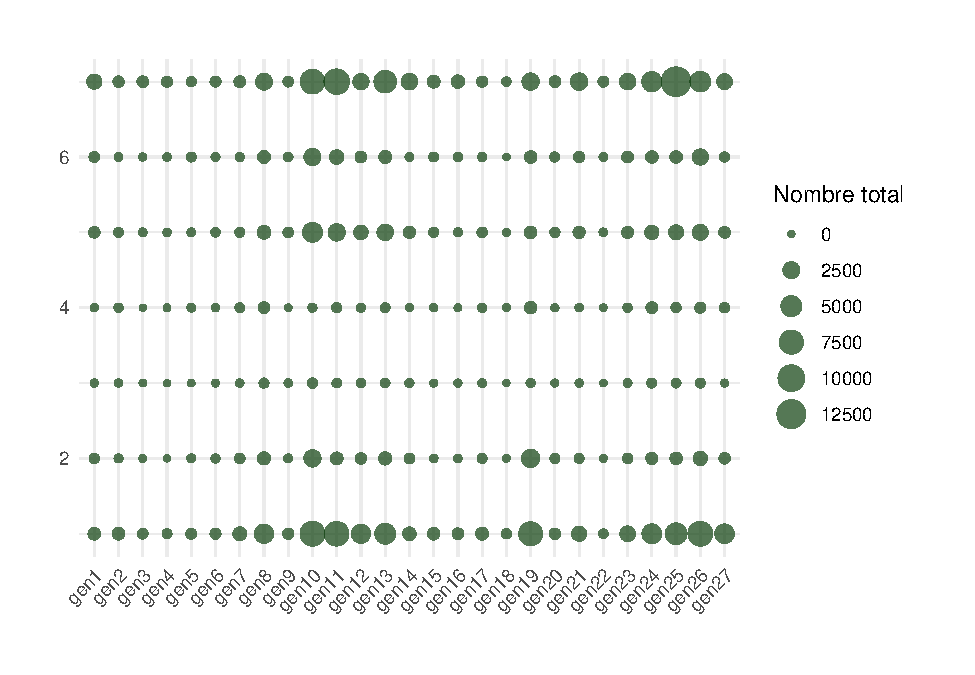
\includegraphics{EL_MAZZOUJI_Wahel_GILLET_Louison_ADM_DM1_files/figure-latex/especes_forest-1} 

}

\caption{Répartition des espèces d'arbres par type forestier}\label{fig:especes_forest}
\end{figure}

Nous remarquons par la figure 1 que les espèces 10,11,25 et 26 semblent
être les plus liées aux types forestiers. En effet, elles sont beaucoup
plus présentes sur les types 1 et 7. A l'inverse, les espèces 2 à 6 ne
semblent pas être liées au type forestier. Cependant, nous verrons après
divers calcul et une analyse plus profonde que notre intuition peut
parfois nous jouer des tours.

Nous voulons donc calculer le \(R^2\) de chaque variable densité de
peuplement où

\[
R^2 = \frac{\text{variance inter-types forestiers}}{\text{variance totale}}
\]

Après calcul, nous isolons les 5 espèces les plus (respectivement moins)
liées aux types :

\begin{longtable}[]{@{}rrrrr@{}}
\caption{R² des 5 espèces les plus liées au type}\tabularnewline
\toprule\noalign{}
gen25 & gen11 & gen2 & gen16 & gen17 \\
\midrule\noalign{}
\endfirsthead
\toprule\noalign{}
gen25 & gen11 & gen2 & gen16 & gen17 \\
\midrule\noalign{}
\endhead
\bottomrule\noalign{}
\endlastfoot
0.1847 & 0.1439 & 0.1325 & 0.1181 & 0.0964 \\
\end{longtable}

\begin{longtable}[]{@{}rrrrr@{}}
\caption{R² des 5 espèces les moins liées au type}\tabularnewline
\toprule\noalign{}
gen6 & gen20 & gen14 & gen18 & gen13 \\
\midrule\noalign{}
\endfirsthead
\toprule\noalign{}
gen6 & gen20 & gen14 & gen18 & gen13 \\
\midrule\noalign{}
\endhead
\bottomrule\noalign{}
\endlastfoot
0.0084 & 0.0139 & 0.0191 & 0.0251 & 0.0303 \\
\end{longtable}

Nous constatons alors que nos premières intuitions étaient plus ou moins
bonnes. En effet, les espèces 25 et 11 sont les plus liées au type
forestier tandis que l'espèce 6 est la moins liée au type forestier. En
revanche, nous avions supposé que l'espèce 2 n'était pas liée au type.
Or, la table 3 nous indique qu'elle est clairement une des espèces la
plus liée au type forestier car environ 13\% de la variabilité de sa
densité de peuplement est expliquée par le type forestier.

Nous devons vérifier que le \(R^2\) de la partition est égal à la
moyenne des \(R^2\) des espèces. Pour cela, nous calculons le \(R^2\)
pour chaque espèce \(j\) :

\[
R^2_{j} = \frac{I_{inter-types,j}}{I_{total,j}}
\]

Puis, nous comparons avec :

\[
R^2_{partition} = \frac{1}{p} \sum_{j=1}^{p} R^2_{j}
\]

où \(p\) est le nombre d'espèces (27).

Nous retrouvons bien informatiquement que le \(R^2\) de la partition est
égal à la moyenne des \(R^2\) des espèces, comme le montre l'extrait de
code suivant :

\begin{Shaded}
\begin{Highlighting}[]
\FunctionTok{print}\NormalTok{(R2)}
\end{Highlighting}
\end{Shaded}

\begin{verbatim}
[1] 0.06884614
\end{verbatim}

\begin{Shaded}
\begin{Highlighting}[]
\FunctionTok{print}\NormalTok{(moyenne\_R2\_especes)}
\end{Highlighting}
\end{Shaded}

\begin{verbatim}
[1] 0.06884614
\end{verbatim}

(le codage des variables est fourni en
\protect\hyperlink{annexe}{Annexe})

\newpage

\hypertarget{partie-2}{%
\section{PARTIE 2}\label{partie-2}}

\hypertarget{pruxe9liminaires}{%
\subsection{Préliminaires}\label{pruxe9liminaires}}

Nous savons que l'espace \(Y\) peut être décomposé de la manière
suivante : \[
\langle Y \rangle = \langle 1 \rangle + \langle Y_{\text{centré}} \rangle
\] où \(\langle 1 \rangle\) est le sous-espace vectoriel engendré par le
vecteur constant \(\mathbf{1}\), et
\(\langle Y_{\text{centré}} \rangle\) représente le sous-espace
vectoriel engendré par \(Y\) une fois centré.

La projection \(\Pi_Y x^j\) peut donc être décomposée comme suit : \[
\Pi_Y x^j = \Pi_1 x^j + \Pi_{Y_{\text{centré}}} x^j
\] où \(\Pi_1 x^j\) est la projection de \(x^j\) sur le vecteur
constant, et \(\Pi_{Y_{\text{centré}}} x^j\) est la projection de
\(x^j\) sur l'espace engendré par les colonnes de \(Y_{\text{centré}}\).

Cependant, la projection sur le vecteur constant, \(\Pi_1 x^j\), est
égale à zéro, car \(x^j\) est une variable centrée. Autrement dit,
lorsque nous projetons \(x^j\) sur le vecteur constant, nous obtenons :
\[
\Pi_1 x^j = 0
\] En substituant cette relation dans l'équation précédente, nous
obtenons : \[
\Pi_Y x^j = 0 + \Pi_{Y_{\text{centré}}} x^j
\] d'où il s'ensuit que : \[
\Pi_Y x^j = \Pi_{Y_{\text{centré}}} x^j
\]

Ainsi, nous avons montré que, pour tout \(j\), la projection de \(x^j\)
sur \(Y\) est égale à la projection de \(x^j\) sur
\(Y_{\text{centré}}\).\newline Le fait que ces deux projections soient
égales signifie que la projection sur cet espace (lié aux types
forestiers) est la même qu'elle soit centrée ou non, car les types
forestiers sont des variables qualitatives représentées par des
indicatrices. Le centrage ne change donc pas le résultat.

On a : \[
\| \Pi_Y x^j \|_W^2 = \langle \Pi_Y x^j, \Pi_Y x^j \rangle_W
\] La projection de \(x^j\) sur \(Y\) est donnée par : \[
\Pi_Y x^j = \sum_{q=1}^{Q} w^q (\overline{x}^q - \overline{x})
\] où \(\overline{x}^q\) est la moyenne pondérée de \(x^j\) pour le type
forestier \(q\), et \(\overline{x}\) est la moyenne globale.

Statistiquement, \(\| \Pi_Y x^j \|_W^2\) représente la variance
inter-groupes de \(x^j\), c'est-à-dire la part de la variance totale de
\(x^j\) qui est expliquée par les types forestiers : \[
\| \Pi_Y x^j \|_W^2 = \sum_{q=1}^{Q} w^q (\overline{x^q} - \overline{x})^2
\]

Cette expression mesure la part de la variabilité de \(x^j\) expliquée
par la partition en types forestiers.

\hypertarget{programmation-et-calcul-de-pi_y-pi_x_j-puis-de-texttrpi_x_j-pi_y}{%
\subsection{\texorpdfstring{Programmation et calcul de \(\Pi_Y\),
\(\Pi_{x_j}\) puis de
\(\text{tr}(\Pi_{x_j} \Pi_Y)\)}{Programmation et calcul de \textbackslash Pi\_Y, \textbackslash Pi\_\{x\_j\} puis de \textbackslash text\{tr\}(\textbackslash Pi\_\{x\_j\} \textbackslash Pi\_Y)}}\label{programmation-et-calcul-de-pi_y-pi_x_j-puis-de-texttrpi_x_j-pi_y}}

\hypertarget{calcul-de-pi_y}{%
\subsubsection{\texorpdfstring{Calcul de
\(\Pi_Y\)}{Calcul de \textbackslash Pi\_Y}}\label{calcul-de-pi_y}}

Le projecteur \(\Pi_Y\) est défini comme le projecteur sur l'espace
généré par les colonnes de la matrice \(Y\). Mathématiquement, il est
formulé comme suit :

\[
   \Pi_Y = Y \left( Y' W Y \right)^{-1} Y' W
   \]

\hypertarget{calcul-de-pi_x_j}{%
\subsubsection{\texorpdfstring{Calcul de
\(\Pi_{x_j}\)}{Calcul de \textbackslash Pi\_\{x\_j\}}}\label{calcul-de-pi_x_j}}

De la même manière, nous avons :

\[
   \Pi_{x_j} = {x_j} \left( {x_j}' W {x_j} \right)^{-1} {x_j}' W
   \]

\hypertarget{calcul-de-texttrpi_x_j-pi_y}{%
\subsubsection{\texorpdfstring{Calcul de
\(\text{tr}(\Pi_{x_j} \Pi_Y)\)}{Calcul de \textbackslash text\{tr\}(\textbackslash Pi\_\{x\_j\} \textbackslash Pi\_Y)}}\label{calcul-de-texttrpi_x_j-pi_y}}

Pour chaque vecteur \(x_j\), le calcul de \(\text{tr}(\Pi_{x_j} \Pi_Y)\)
implique la projection de \(x_j\) dans l'espace défini par \(Y\). Cette
opération nous permet d'évaluer la quantité de variabilité dans \(x_j\)
qui est expliquée par la classification en types forestiers. Ainsi,

\[ 
\begin{aligned} 
\text{tr}(\Pi_{x_j} \Pi_Y) & = \text{tr} ({x_j} \left( {x_j}' W {x_j} \right)^{-1} {x_j}' W \Pi_Y) \\
& = \left( {x_j}' W {x_j} \right)^{-1} \text{tr} ({x_j}{x_j}' W \Pi_Y)\\
& = \frac{1}{\|x_j\|^2}  \text{tr} ({x_j}' W \Pi_Y{x_j})\\
& = \frac{1}{\|x_j\|^2}  \langle x_j, \Pi_Y x_j \rangle_W \\
& = \frac{\|\Pi_Y x_j\|_W^2}{\|x_j\|^2}\\
& = R^2({x_j} \mid Y)
\end{aligned}
\]

où \(R^2(x_j \mid Y)\) représente la part de variabilité de \({x_j}\)
qui est due à Y. En somme, \(\text{tr}(\Pi_{x_j} \Pi_Y)\) mesure la part
de variabilité des densités d'une espèce due au type forestier.

\begin{longtable}[]{@{}rrrrrr@{}}
\caption{R² des espèces selon le type forestier par calcul de la
trace}\tabularnewline
\toprule\noalign{}
gen2 & gen6 & gen11 & gen14 & gen20 & gen25 \\
\midrule\noalign{}
\endfirsthead
\toprule\noalign{}
gen2 & gen6 & gen11 & gen14 & gen20 & gen25 \\
\midrule\noalign{}
\endhead
\bottomrule\noalign{}
\endlastfoot
0.1327 & 0.0085 & 0.1441 & 0.0191 & 0.0139 & 0.1849 \\
\end{longtable}

Nous retrouvons alors les mêmes \(R^2\) que dans la première partie.
(les minimes différences sont dues aux arrondis)

\hypertarget{calcul-de-texttrr-pi_y-et-interpruxe9tation-statistique}{%
\subsection{\texorpdfstring{Calcul de \(\text{tr}(R \Pi_Y)\) et
interprétation
statistique}{Calcul de \textbackslash text\{tr\}(R \textbackslash Pi\_Y) et interprétation statistique}}\label{calcul-de-texttrr-pi_y-et-interpruxe9tation-statistique}}

On note \[ R = X M X' W \].

Alors \(\text{tr}(R \Pi_Y)\) représente la somme des variances
expliquées par la partition en types forestiers, comme représenté par
\(Y\), sur l'ensemble des variables contenues dans la matrice \(X\).
Cette valeur constitue une mesure de l'inertie inter-types forestiers et
fournit une indication globale de la quantité d'information expliquée
par la classification des types forestiers sur l'ensemble des variables
analysées. Après calcul, nous obtenons \(\text{tr}(R \Pi_Y) =\)
0.0688461. Nous retrouvons alors la proportion de variance expliquée par
les types forestiers dans la variabilité des densités de peuplement
obtenue dans la première partie.

\hypertarget{calcul-de-texttrpi_x_j-pi_z-texttrr-pi_z-et-interpruxe9tation-statistique}{%
\subsection{\texorpdfstring{Calcul de \(\text{tr}(\Pi_{x_j} \Pi_Z)\),
\(\text{tr}(R \Pi_Z)\) et interprétation
statistique}{Calcul de \textbackslash text\{tr\}(\textbackslash Pi\_\{x\_j\} \textbackslash Pi\_Z), \textbackslash text\{tr\}(R \textbackslash Pi\_Z) et interprétation statistique}}\label{calcul-de-texttrpi_x_j-pi_z-texttrr-pi_z-et-interpruxe9tation-statistique}}

Le projecteur \(\Pi_Z\) est défini sur l'espace des indicatrices de
sols, représentées par la matrice \(Z\). Le calcul de
\(\text{tr}(\Pi_{x_j} \Pi_Z)\) permet d'évaluer combien de la
variabilité de \(x_j\) est expliquée par la partition en types de sols.
La formule correspondante est :

\[
\text{tr}(\Pi_{x_j} \Pi_Z) = \text{tr} ({x_j} \left( {x_j}' W {x_j} \right)^{-1} {x_j}' W \Pi_Z) = R^2({x_j} \mid Z)
\]

\begin{longtable}[]{@{}rrrrrr@{}}
\caption{R² des espèces selon le type de sol par calcul de la
trace}\tabularnewline
\toprule\noalign{}
gen2 & gen6 & gen11 & gen14 & gen20 & gen25 \\
\midrule\noalign{}
\endfirsthead
\toprule\noalign{}
gen2 & gen6 & gen11 & gen14 & gen20 & gen25 \\
\midrule\noalign{}
\endhead
\bottomrule\noalign{}
\endlastfoot
0.0175 & 0.0088 & 0.0673 & 0.0317 & 0.0044 & 0.3233 \\
\end{longtable}

Cet extrait nous montre par exemple qu'environ 32\% de la variabilité
des densités de peuplement de l'espèce 25 est expliquée par le type de
sol.

En parallèle, \(\text{tr}(R \Pi_Z)\) quantifie la somme des variances
expliquées par la partition en types de sols sur toutes les variables
dans \(X\). Cette valeur constitue une mesure de l'inertie inter-sols et
fournit une indication globale de la quantité d'information expliquée
par la classification des sols sur l'ensemble des variables analysées.
Le calcul de \(\text{tr}(R \Pi_Z)\) nous donne 0.0758867 soit environ
7,6\%, ce qui est légèrement plus que l'inertie inter-types forestiers.
Ainsi, la classification des sols sur l'ensemble des variables analysées
nous fournit un peu plus d'informations que la classification des types
forestiers.

\hypertarget{conclusion}{%
\section{CONCLUSION}\label{conclusion}}

Cette analyse nous a permis de mieux comprendre les dynamiques de
peuplement forestier dans la forêt du bassin du Congo. En intégrant des
approches statistiques robustes, nous avons pu quantifier la variabilité
des espèces et leur répartition en fonction des types forestiers. Les
résultats de cette étude fourniront des bases solides pour des
recherches futures et des actions de conservation.

\newpage

\hypertarget{annexe}{%
\section{ANNEXE : CODE R}\label{annexe}}

\begin{Shaded}
\begin{Highlighting}[]
\CommentTok{\# En tête {-}{-}{-}{-}}

\CommentTok{\# Desc : DM1 ADM Date: 02/10/2024 Auteur : EL MAZZOUJI Wahel \& GILLET Louison}

\CommentTok{\# Dataframe {-}{-}{-}{-}}

\NormalTok{Datagenus }\OtherTok{\textless{}{-}} \FunctionTok{read.csv}\NormalTok{(}\StringTok{"data/Datagenus.csv"}\NormalTok{, }\AttributeTok{sep =} \StringTok{";"}\NormalTok{)}
\NormalTok{data }\OtherTok{\textless{}{-}}\NormalTok{ Datagenus[}\DecValTok{1}\SpecialCharTok{:}\DecValTok{1000}\NormalTok{, ]  }\CommentTok{\# On ne prend pas la ligne 1001 }
\NormalTok{especes }\OtherTok{\textless{}{-}} \FunctionTok{paste0}\NormalTok{(}\StringTok{"gen"}\NormalTok{, }\DecValTok{1}\SpecialCharTok{:}\DecValTok{27}\NormalTok{)}
\NormalTok{colonnes\_selectionnees }\OtherTok{\textless{}{-}} \FunctionTok{c}\NormalTok{(especes, }\StringTok{"surface"}\NormalTok{, }\StringTok{"forest"}\NormalTok{, }\StringTok{"geology"}\NormalTok{)}
\NormalTok{data }\OtherTok{\textless{}{-}}\NormalTok{ data[, colonnes\_selectionnees]}

\CommentTok{\# Partie 1 {-}{-}{-}{-} 1.1 Calcul de la densité de peuplement pour chaque espèce (gen1}
\CommentTok{\# à gen27) \#\#\#\#}

\NormalTok{densite\_peuplement }\OtherTok{\textless{}{-}} \FunctionTok{as.matrix}\NormalTok{(data[especes]}\SpecialCharTok{/}\NormalTok{data}\SpecialCharTok{$}\NormalTok{surface)  }\CommentTok{\# Conversion en matrice }

\DocumentationTok{\#\#\#\# 1.2 Centrage et réduction avec des opérations matricielles \#\#\#\#}

\DocumentationTok{\#\#\# Calcul des moyennes pour chaque espèce (colonne)}

\NormalTok{moyennes\_especes }\OtherTok{\textless{}{-}}\NormalTok{ (}\FunctionTok{colMeans}\NormalTok{(densite\_peuplement))}

\DocumentationTok{\#\#\# Calcul des écarts{-}types pour chaque espèce (colonne)}
\NormalTok{n }\OtherTok{\textless{}{-}} \FunctionTok{nrow}\NormalTok{(densite\_peuplement)}
\NormalTok{p }\OtherTok{\textless{}{-}} \FunctionTok{ncol}\NormalTok{(densite\_peuplement)}
\NormalTok{mat\_moyenne }\OtherTok{\textless{}{-}} \FunctionTok{matrix}\NormalTok{(moyennes\_especes, }\AttributeTok{nrow =}\NormalTok{ n, }\AttributeTok{ncol =}\NormalTok{ p, }\AttributeTok{byrow =} \ConstantTok{TRUE}\NormalTok{)}
\CommentTok{\# remplit chaque ligne avec la densité de la colonne}

\NormalTok{sd\_especes }\OtherTok{\textless{}{-}} \FunctionTok{sqrt}\NormalTok{(}\FunctionTok{colSums}\NormalTok{((densite\_peuplement }\SpecialCharTok{{-}}\NormalTok{ mat\_moyenne)}\SpecialCharTok{\^{}}\DecValTok{2}\NormalTok{)}\SpecialCharTok{/}\NormalTok{(n }\SpecialCharTok{{-}} \DecValTok{1}\NormalTok{))  }\CommentTok{\#racine de la variance sans{-}biais }

\DocumentationTok{\#\#\# Centrage et réduction : on soustrait les moyennes et on divise par}
\DocumentationTok{\#\#\# l\textquotesingle{}écart{-}type}

\NormalTok{mat\_sd }\OtherTok{\textless{}{-}} \FunctionTok{matrix}\NormalTok{(sd\_especes, }\AttributeTok{nrow =}\NormalTok{ n, }\AttributeTok{ncol =}\NormalTok{ p, }\AttributeTok{byrow =} \ConstantTok{TRUE}\NormalTok{)}
\CommentTok{\# idem avec l\textquotesingle{}écart{-}type}

\NormalTok{densite\_centree\_reduite }\OtherTok{\textless{}{-}}\NormalTok{ (densite\_peuplement }\SpecialCharTok{{-}}\NormalTok{ mat\_moyenne)}\SpecialCharTok{/}\NormalTok{mat\_sd}

\DocumentationTok{\#\#\#\# 1.3 Barycentre et inertie \#\#\#\#}

\DocumentationTok{\#\#\# 1.3.1 Barycentre à l\textquotesingle{}origine (moyennes des colonnes proches de 0)}
\DocumentationTok{\#\#\# summary(densite\_centree\_reduite)}
\NormalTok{moyennes\_apres\_centrage }\OtherTok{\textless{}{-}} \FunctionTok{colMeans}\NormalTok{(densite\_centree\_reduite)}
\NormalTok{test\_barycentre\_a\_l\_origine }\OtherTok{\textless{}{-}} \FunctionTok{all}\NormalTok{(}\FunctionTok{abs}\NormalTok{(moyennes\_apres\_centrage) }\SpecialCharTok{\textless{}} \FloatTok{1e{-}10}\NormalTok{)}

\DocumentationTok{\#\#\# 1.3.2 Inertie totale (variances des colonnes proches de 1) Variance par}
\DocumentationTok{\#\#\# colonne}
\NormalTok{variances\_apres\_centrage }\OtherTok{\textless{}{-}} \FunctionTok{colSums}\NormalTok{(densite\_centree\_reduite}\SpecialCharTok{\^{}}\DecValTok{2}\NormalTok{)}\SpecialCharTok{/}\NormalTok{(n }\SpecialCharTok{{-}} \DecValTok{1}\NormalTok{)}

\CommentTok{\# Inertie totale = somme des variances}
\NormalTok{inertie\_totale }\OtherTok{\textless{}{-}} \FunctionTok{sum}\NormalTok{(variances\_apres\_centrage)}

\DocumentationTok{\#\#\#\# 2.1 Calcul des poids, barycentres des types forestiers et normes}
\DocumentationTok{\#\#\#\# euclidiennes de ces barycentres \#\#\#\#}

\DocumentationTok{\#\#\# Identification des types forestiers}
\NormalTok{types\_forestiers }\OtherTok{\textless{}{-}} \FunctionTok{unique}\NormalTok{(data}\SpecialCharTok{$}\NormalTok{forest)}

\DocumentationTok{\#\#\# Création d\textquotesingle{}une matrice pour les poids, barycentres et normes euclidiennes}
\DocumentationTok{\#\#\# carrées}
\NormalTok{d }\OtherTok{\textless{}{-}} \FunctionTok{length}\NormalTok{(types\_forestiers)}
\NormalTok{poids\_forestiers }\OtherTok{\textless{}{-}} \FunctionTok{numeric}\NormalTok{(d)}
\NormalTok{barycentres\_forestiers }\OtherTok{\textless{}{-}} \FunctionTok{matrix}\NormalTok{(}\DecValTok{0}\NormalTok{, }\AttributeTok{nrow =}\NormalTok{ d, }\AttributeTok{ncol =}\NormalTok{ p)  }\CommentTok{\#p=ncol(densite\_centree\_reduite)}
\NormalTok{normes\_euclidiennes\_carre }\OtherTok{\textless{}{-}} \FunctionTok{numeric}\NormalTok{(d)}

\DocumentationTok{\#\#\# Calcul par opérations matricielles}

\ControlFlowTok{for}\NormalTok{ (i }\ControlFlowTok{in} \DecValTok{1}\SpecialCharTok{:}\NormalTok{d) \{}
    \CommentTok{\# Filtrer les parcelles appartenant à chaque type forestier}
\NormalTok{    parcelles\_type\_forestier }\OtherTok{\textless{}{-}}\NormalTok{ densite\_centree\_reduite[data}\SpecialCharTok{$}\NormalTok{forest }\SpecialCharTok{==}\NormalTok{ types\_forestiers[i],}
\NormalTok{        ]}

    \CommentTok{\# Calculer le poids : proportion des parcelles de ce type}
\NormalTok{    poids\_forestiers[i] }\OtherTok{\textless{}{-}} \FunctionTok{nrow}\NormalTok{(parcelles\_type\_forestier)}\SpecialCharTok{/}\FunctionTok{nrow}\NormalTok{(densite\_centree\_reduite)}

    \CommentTok{\# Calcul du barycentre pour chaque type forestier (moyenne par espèce)}
\NormalTok{    barycentres\_forestiers[i, ] }\OtherTok{\textless{}{-}} \FunctionTok{colMeans}\NormalTok{(parcelles\_type\_forestier)}

    \CommentTok{\# Calcul de la norme euclidienne carrée pour chaque type forestier}
\NormalTok{    normes\_euclidiennes\_carre[i] }\OtherTok{\textless{}{-}} \FunctionTok{sum}\NormalTok{(barycentres\_forestiers[i, ]}\SpecialCharTok{\^{}}\DecValTok{2}\NormalTok{)}
\NormalTok{\}}

\DocumentationTok{\#\#\#\# 2.2 Calcul de l\textquotesingle{}inertie inter{-}types et du R2 (coefficient de}
\DocumentationTok{\#\#\#\# détermination) \#\#\#\#}

\DocumentationTok{\#\#\# Inertie inter{-}types}
\NormalTok{inertie\_inter\_types }\OtherTok{\textless{}{-}} \FunctionTok{sum}\NormalTok{(poids\_forestiers }\SpecialCharTok{*}\NormalTok{ normes\_euclidiennes\_carre)}

\DocumentationTok{\#\#\# Coefficient de détermination R2}
\NormalTok{R2 }\OtherTok{\textless{}{-}}\NormalTok{ inertie\_inter\_types}\SpecialCharTok{/}\NormalTok{inertie\_totale}

\DocumentationTok{\#\#\#\# 2.3 Pourcentage d\textquotesingle{}information (variabilité du peuplement) \#\#\#\#}
\NormalTok{pourcentage\_information }\OtherTok{\textless{}{-}}\NormalTok{ R2 }\SpecialCharTok{*} \DecValTok{100}

\DocumentationTok{\#\#\#\# 3.1 Calcul de la variance totale et de la variance inter{-}types pour chaque}
\DocumentationTok{\#\#\#\# espèce \#\#\#\#}

\DocumentationTok{\#\#\# Variance totale}
\NormalTok{variance\_totale\_par\_espece }\OtherTok{\textless{}{-}} \FunctionTok{colSums}\NormalTok{(densite\_centree\_reduite}\SpecialCharTok{\^{}}\DecValTok{2}\NormalTok{)}\SpecialCharTok{/}\NormalTok{(n }\SpecialCharTok{{-}} \DecValTok{1}\NormalTok{)}

\DocumentationTok{\#\#\# Variance inter{-}types}
\NormalTok{variance\_inter\_types\_par\_espece }\OtherTok{\textless{}{-}} \FunctionTok{numeric}\NormalTok{(}\FunctionTok{ncol}\NormalTok{(densite\_centree\_reduite))}

\CommentTok{\# Boucle pour chaque espèce}
\ControlFlowTok{for}\NormalTok{ (j }\ControlFlowTok{in} \DecValTok{1}\SpecialCharTok{:}\FunctionTok{ncol}\NormalTok{(densite\_centree\_reduite)) \{}
    \CommentTok{\# On calcule la variance inter{-}types pour l\textquotesingle{}espèce j}
\NormalTok{    variance\_inter\_types\_par\_espece[j] }\OtherTok{\textless{}{-}} \FunctionTok{sum}\NormalTok{(poids\_forestiers }\SpecialCharTok{*}\NormalTok{ (barycentres\_forestiers[,}
\NormalTok{        j]}\SpecialCharTok{\^{}}\DecValTok{2}\NormalTok{))}
\NormalTok{\}}

\DocumentationTok{\#\#\#\# 3.2 Calcul du R2 pour chaque espèce \#\#\#\#}
\NormalTok{R2\_par\_espece }\OtherTok{\textless{}{-}}\NormalTok{ variance\_inter\_types\_par\_espece}\SpecialCharTok{/}\NormalTok{variance\_totale\_par\_espece}

\DocumentationTok{\#\#\#\# 3.3 Identification des espèces les plus et les moins liées au type}
\DocumentationTok{\#\#\#\# forestier \#\#\#\#}
\NormalTok{especes\_most\_liees }\OtherTok{\textless{}{-}}\NormalTok{ (}\FunctionTok{sort}\NormalTok{(R2\_par\_espece, }\AttributeTok{decreasing =} \ConstantTok{TRUE}\NormalTok{))[}\DecValTok{1}\SpecialCharTok{:}\DecValTok{5}\NormalTok{]  }\CommentTok{\# Les 5 espèces les plus liées}
\NormalTok{especes\_least\_liees }\OtherTok{\textless{}{-}}\NormalTok{ (}\FunctionTok{sort}\NormalTok{(R2\_par\_espece, }\AttributeTok{decreasing =} \ConstantTok{FALSE}\NormalTok{))[}\DecValTok{1}\SpecialCharTok{:}\DecValTok{5}\NormalTok{]  }\CommentTok{\# Les 5 espèces les moins liées}

\DocumentationTok{\#\#\#\# 3.4 Calcul de la moyenne arithmétique des R2 des espèces \#\#\#\#}
\NormalTok{moyenne\_R2\_especes }\OtherTok{\textless{}{-}} \FunctionTok{mean}\NormalTok{(R2\_par\_espece)}

\DocumentationTok{\#\#\#\# 3.5 Vérification que le R2 de la partition est égal à la moyenne des R2}
\DocumentationTok{\#\#\#\# des variables \#\#\#\#}
\NormalTok{verification\_R2 }\OtherTok{\textless{}{-}}\NormalTok{ R2 }\SpecialCharTok{==}\NormalTok{ moyenne\_R2\_especes}

\CommentTok{\# Partie 2 {-}{-}{-}{-} 1.1 Calcul Projection Y \#\#\#\#}

\DocumentationTok{\#\#\# 1.1.1 Préliminaires : création des matrices}
\NormalTok{X }\OtherTok{\textless{}{-}}\NormalTok{ densite\_centree\_reduite}
\FunctionTok{dim}\NormalTok{(X)}
\NormalTok{Y }\OtherTok{\textless{}{-}} \FunctionTok{model.matrix}\NormalTok{(}\SpecialCharTok{\textasciitilde{}}\FunctionTok{as.factor}\NormalTok{(forest) }\SpecialCharTok{{-}} \DecValTok{1}\NormalTok{, }\AttributeTok{data =}\NormalTok{ data)}
\FunctionTok{colnames}\NormalTok{(Y) }\OtherTok{\textless{}{-}} \FunctionTok{paste}\NormalTok{(}\StringTok{"type"}\NormalTok{, }\FunctionTok{seq\_along}\NormalTok{(}\FunctionTok{levels}\NormalTok{(}\FunctionTok{as.factor}\NormalTok{(data}\SpecialCharTok{$}\NormalTok{forest))))}
\NormalTok{W }\OtherTok{\textless{}{-}} \FunctionTok{diag}\NormalTok{(}\DecValTok{1}\SpecialCharTok{/}\NormalTok{n, n, n)  }\CommentTok{\# Matrice de poids équipondérés}
\NormalTok{M }\OtherTok{\textless{}{-}} \FunctionTok{diag}\NormalTok{(}\DecValTok{1}\SpecialCharTok{/}\NormalTok{p, p, p)  }\CommentTok{\# Matrice de poids pour les variables}

\DocumentationTok{\#\#\# 1.1.2 Calcul}
\NormalTok{Pi\_Y }\OtherTok{\textless{}{-}}\NormalTok{ Y }\SpecialCharTok{\%*\%} \FunctionTok{solve}\NormalTok{(}\FunctionTok{t}\NormalTok{(Y) }\SpecialCharTok{\%*\%}\NormalTok{ W }\SpecialCharTok{\%*\%}\NormalTok{ Y) }\SpecialCharTok{\%*\%} \FunctionTok{t}\NormalTok{(Y) }\SpecialCharTok{\%*\%}\NormalTok{ W  }\CommentTok{\#solve donne l\textquotesingle{}inverse de Y\textquotesingle{}WY }


\DocumentationTok{\#\#\#\# 1.2 Calcul Pi\_xj et tr(Pi\_Y*Pi\_xj \#\#\#\#}
\NormalTok{tr\_Pi\_xj\_PiY }\OtherTok{\textless{}{-}} \FunctionTok{numeric}\NormalTok{(p)}

\ControlFlowTok{for}\NormalTok{ (j }\ControlFlowTok{in} \DecValTok{1}\SpecialCharTok{:}\NormalTok{p) \{}
\NormalTok{    x\_j }\OtherTok{\textless{}{-}}\NormalTok{ X[, j]}
\NormalTok{    Pi\_xj }\OtherTok{\textless{}{-}}\NormalTok{ x\_j }\SpecialCharTok{\%*\%} \FunctionTok{solve}\NormalTok{(}\FunctionTok{t}\NormalTok{(x\_j) }\SpecialCharTok{\%*\%}\NormalTok{ W }\SpecialCharTok{\%*\%}\NormalTok{ x\_j) }\SpecialCharTok{\%*\%} \FunctionTok{t}\NormalTok{(x\_j) }\SpecialCharTok{\%*\%}\NormalTok{ W}
\NormalTok{    tr\_Pi\_xj\_PiY[j] }\OtherTok{\textless{}{-}} \FunctionTok{sum}\NormalTok{(}\FunctionTok{diag}\NormalTok{(Pi\_xj }\SpecialCharTok{\%*\%}\NormalTok{ Pi\_Y))}
\NormalTok{\}}
\FunctionTok{sum}\NormalTok{(tr\_Pi\_xj\_PiY)}

\DocumentationTok{\#\#\#\# 1.3 Calcul de tr(RPI\_Y)}
\NormalTok{R }\OtherTok{\textless{}{-}}\NormalTok{ X }\SpecialCharTok{\%*\%}\NormalTok{ M }\SpecialCharTok{\%*\%} \FunctionTok{t}\NormalTok{(X) }\SpecialCharTok{\%*\%}\NormalTok{ W}
\NormalTok{trace\_R\_Pi\_Y }\OtherTok{\textless{}{-}} \FunctionTok{sum}\NormalTok{(}\FunctionTok{diag}\NormalTok{(R }\SpecialCharTok{\%*\%}\NormalTok{ Pi\_Y))}

\DocumentationTok{\#\#\#\# 2.1 Calcul de tr(Pi\_xj*Pi\_Z) \#\#\#\#}

\DocumentationTok{\#\#\# 2.1.1 Création matrice Z}
\NormalTok{Z }\OtherTok{\textless{}{-}} \FunctionTok{model.matrix}\NormalTok{(}\SpecialCharTok{\textasciitilde{}}\FunctionTok{as.factor}\NormalTok{(geology) }\SpecialCharTok{{-}} \DecValTok{1}\NormalTok{, }\AttributeTok{data =}\NormalTok{ data)}
\FunctionTok{colnames}\NormalTok{(Z) }\OtherTok{\textless{}{-}} \FunctionTok{paste0}\NormalTok{(}\StringTok{"geology"}\NormalTok{, }\FunctionTok{setdiff}\NormalTok{(}\DecValTok{1}\SpecialCharTok{:}\DecValTok{6}\NormalTok{, }\DecValTok{4}\NormalTok{))  }\CommentTok{\#il n\textquotesingle{}y a pas de 4 pour geology }

\DocumentationTok{\#\#\# 2.1.2 Calcul Pi\_Z}
\NormalTok{Pi\_Z }\OtherTok{\textless{}{-}}\NormalTok{ Z }\SpecialCharTok{\%*\%} \FunctionTok{solve}\NormalTok{(}\FunctionTok{t}\NormalTok{(Z) }\SpecialCharTok{\%*\%}\NormalTok{ W }\SpecialCharTok{\%*\%}\NormalTok{ Z) }\SpecialCharTok{\%*\%} \FunctionTok{t}\NormalTok{(Z) }\SpecialCharTok{\%*\%}\NormalTok{ W}

\DocumentationTok{\#\#\# 2.1.3 Calcul}
\NormalTok{tr\_Pi\_xj\_PiZ }\OtherTok{\textless{}{-}} \FunctionTok{numeric}\NormalTok{(p)}

\ControlFlowTok{for}\NormalTok{ (j }\ControlFlowTok{in} \DecValTok{1}\SpecialCharTok{:}\NormalTok{p) \{}
\NormalTok{    x\_j }\OtherTok{\textless{}{-}}\NormalTok{ X[, j]}
\NormalTok{    Pi\_x\_j }\OtherTok{\textless{}{-}}\NormalTok{ x\_j }\SpecialCharTok{\%*\%} \FunctionTok{solve}\NormalTok{(}\FunctionTok{t}\NormalTok{(x\_j) }\SpecialCharTok{\%*\%}\NormalTok{ W }\SpecialCharTok{\%*\%}\NormalTok{ x\_j) }\SpecialCharTok{\%*\%} \FunctionTok{t}\NormalTok{(x\_j) }\SpecialCharTok{\%*\%}\NormalTok{ W}
\NormalTok{    tr\_Pi\_xj\_PiZ[j] }\OtherTok{\textless{}{-}} \FunctionTok{sum}\NormalTok{(}\FunctionTok{diag}\NormalTok{(Pi\_x\_j }\SpecialCharTok{\%*\%}\NormalTok{ Pi\_Z))  }\CommentTok{\# trace(Pi\_x\_j * Pi\_Z)}
\NormalTok{\}}

\DocumentationTok{\#\#\#\# 2.2 Calcul de tr(RPi\_Z) \#\#\#\#}
\NormalTok{tr\_R\_Pi\_Z }\OtherTok{\textless{}{-}} \FunctionTok{sum}\NormalTok{(}\FunctionTok{diag}\NormalTok{(R }\SpecialCharTok{\%*\%}\NormalTok{ Pi\_Z))}

\CommentTok{\# Sauvegarde pour Rmd {-}{-}{-}{-}}
\FunctionTok{save.image}\NormalTok{(}\AttributeTok{file =} \StringTok{"ressources/prepa.RData"}\NormalTok{)}
\end{Highlighting}
\end{Shaded}


\end{document}
